\documentclass[a4paper, 11pt]{article}

\usepackage{fullpage, graphicx, float, tabulary, multirow, multicol, lscape, hyperref}

\setcounter{tocdepth}{2}

\begin{document}

\title{CS124 Individual Project - Drown The Scurvy Dog - Write-Up}
\author{Nic Dart (nid21@aber.ac.uk)}
\date{May 2014}

\maketitle

\newpage

\tableofcontents

\newpage

\section{Analysis}

\subsection{Problem and Solution Spaces}

The problem space for this assignment was defined in the original project specification, which can be found on the University's BlackBoard Online Learning Environment. A quote of the problem space from the above specification is below:

\begin{quote}
This project is a variation of hangman. It involves programming both a text based, and a graphics based version of the same game. The graphics based version should be pirate themed. The words to be guessed must be pirate themed and must be read from the provided file called piratewords.txt that has the format (you can add to the phrases: see http://www.yarr.org.uk/talk/)
\end{quote}

I have defined the solution space to encompass the whole of the problem space, as well as to include some of the suggested advanced functionality and features of my own. This is because I believe I will be able to provide an accurate and reliable implementation of the application defined in the original specification and by providing additional functionality will not hinder the application's performance.

\subsection{Application Requirements}

After reading through the original specification, I have decided that the application has the following functional requirements:

\begin{enumerate}
\item Present a graphical and command line interface which allows a user to play a game of 'Drown The Scurvy Dog' and do the following:
\begin{enumerate}
\item Add or delete words or phrases to the dictionary
\item Save, load or reload the dictionary file
\item View all phrases and words
\item View an animated representation of the game
\item Play complete and abandon games
\end{enumerate}
\item Utilize a human readable storage format
\item I have decided to use Json as the storage format as it is a standardized notation/structure and is still human readable
\end{enumerate}

As well as the above functional requirements, I have also established a number of aesthetic and non-functional requirements:

\begin{enumerate}
\setcounter{enumi}{3}
\item The graphical interfaces provided by the application should contain menu bars and tool bars, similar to a traditional WIMP application
\begin{enumerate}
\item The menus and menu items should be appropriately labeled
\item Menu Items should be placed under the relevant headings
\end{enumerate}
\item There should be a status bar where guessed letters and the word to be guessed should be shown, along with an input box, submit button and number of lives left.
\item The graphical interfaces should not have different input fields for a single character or whole word (as this is easily detected)
\item The graphic display should take up the majority of the space, providing a large, picture or vector graphic based view of the state of the game
\end{enumerate}

I have represented the requirements laid out above as a Use Case Diagram (\ref{UseCaseDiagram}) on page \pageref{UseCaseDiagram}.

\subsection{Running Environment}

From the specification I can determine several factors about the environment my implementation will be run in. I am also making several assumptions about the environment based on what information I haven't been told:

\begin{enumerate}
\item The application will be run using Java 1.7 (OpenJDK 7) as OpenJDK8 is not available in the package repository of my operating system. 
\item The application will be run on a platform which supports the Java Swing library
\item I cannot assume what Operating System the application will be run on, therefore it should be compatible with all major Operating Systems: Windows, Macintosh OS X, and Linux
\item The application could conceivably be run as a Jar
\end{enumerate}

\subsection{My Solution}

I plan on implementing a solution using MVC design patters, I considered using Observer/Observable but there is a two way exchange of data to/from the View which would make an Observer/Observable approach impracticable as the View and Model would both have to be an Observer and Observable of each other. This solution allows me to separate out the view from the underlying models/work to allow rewriting/changes/replacement of the view with minimal to no changes of the model. This also gives me the added easy implementation of the two Views specified in the brief. 

The controllers will be the EventListener for the Swing graphical view, but for the Command line view they will be rolled into the view, as there is little or need or practicality of separating out the controllers. 

My decision to use Json as the storage format instead of the provided format was to keep the data standardized and easy to manipulate by hand, the provided format was clumsy because editing it required you to add the desired elements and then edit the total number of elements in that section, whilst easy when adding/deleting in small numbers of words or phrases, or altering an existing word, larger numbers of additions/deletions would be more time consuming and would result in parsing errors if the number of words/phrases at the beginning was incorrect. 

\begin{figure}[H]
\centering
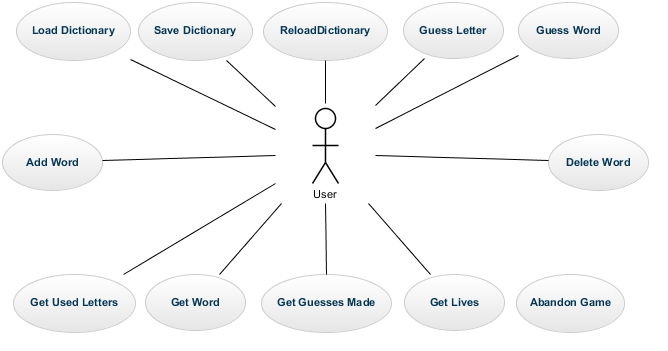
\includegraphics[scale=0.6]{./res/UsecaseDiagram.jpg}
\caption{Use Case Diagram}
\label{UseCaseDiagram}
\end{figure}


\newpage

\section{Design}

\subsection{Model Design}

\begin{figure}[H]
\centering
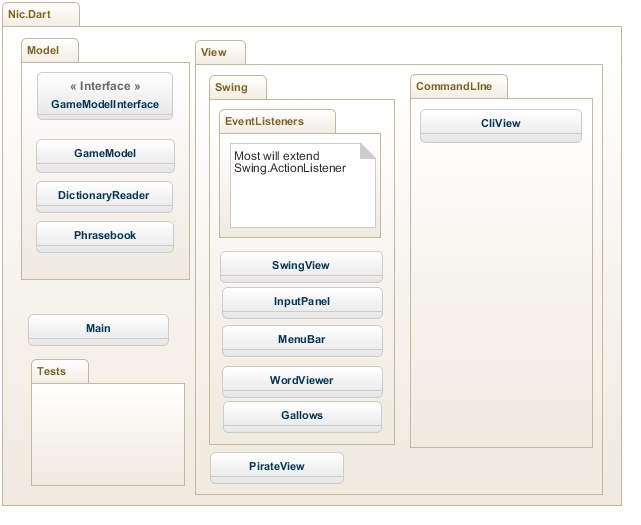
\includegraphics[scale=0.7]{./res/PackageDiagram.jpg}
\caption{Package Diagram}
\label{PackageDiagram}
\end{figure}


\begin{figure}[H]
\centering
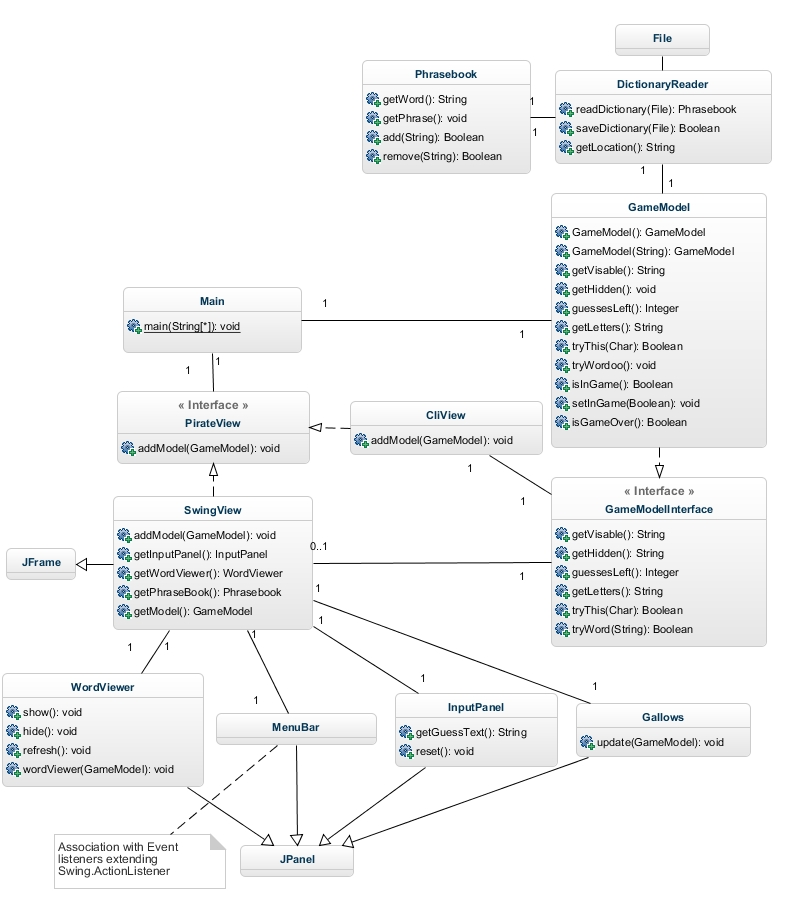
\includegraphics[scale=0.6]{./res/ClassDiagram.jpg}
\caption{Class Diagram}
\label{ModelClassDiagram}
\end{figure}

Following MVC guidelines, I have split the views and the models up, in the \texttt{Main} class, the \texttt{Model} is created, and then passed to the \texttt{View} that the user has chosen. the \texttt{PirateView} interface contains one method; \texttt{addModel} which takes a \texttt{Model} and associates it with the view. I designed it this way so the view can retrieve data from the model when necessary, as there is no need for the model to notify the \texttt{View} of a change as changes only happen when new data has been entered, and the \texttt{View} can then make method calls to the \texttt{Model} to do guesses. 

The \texttt{PhraseBook} class holds the associated pirate words and phrases, it is the thing that is (de)serialized to/from Json in the dictionary.json file. The \texttt{DictionaryReader} class only serves to read from a file and return a \texttt{PhraseBook} object, or take a \texttt{PhraseBook} object and a file location and serialize and write the \texttt{PhraseBook} to Json.

The \texttt{SwingView} and \texttt{CliView} which both implement \texttt{PirateView} are the Views (and Controllers) for the Model. I decided to separate the \texttt{ActionListeners} out from the \texttt{SwingView} so as to not have many classes or anonymous classes in the associated \texttt{SwingView} elements. However for the \texttt{CliView} as there is significantly less code required to create visual elements, I opted to keep the Controllers within the class, as separating them would only make using it more cumbersome. 

\subsection{Graphical User Interface Design}

A loose design was provided for us in the brief, both for Swing and Cli, however the brief said `might look like', so some creative freedom was implied. I decided to simplify the design to make it slightly more user friendly, my initial designs were as follows:

\begin{figure}[H]
\centering
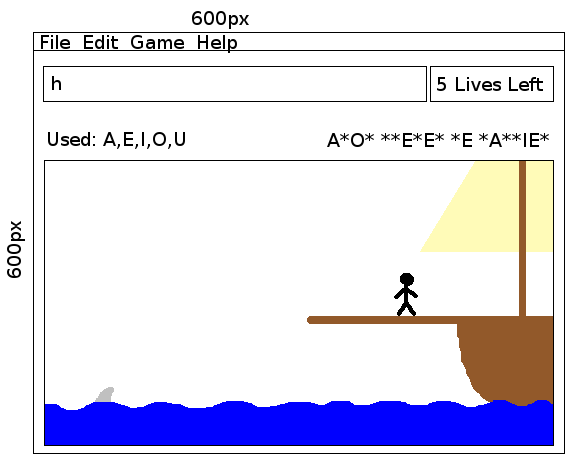
\includegraphics[scale=0.5]{./res/SwingViewDesign.png}
\caption{Swing View Initial Design}
\label{SwingView}
\end{figure}

The File menu will hold options for loading and saving the dictionary file, Edit will hold options for adding and deleting words from the game, as well as viewing a list of phrases and words in the game, and lastly Game will hold options for abandoning the game or getting hints.

\begin{figure}[H]
\centering
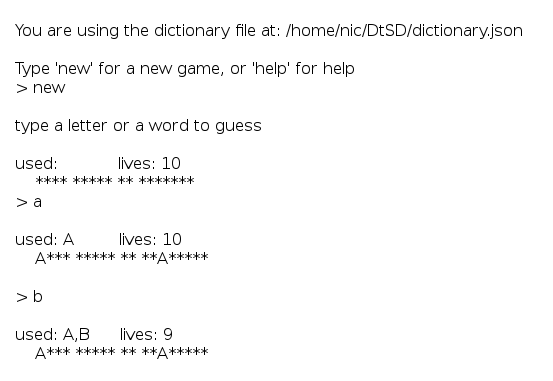
\includegraphics[scale=0.75]{./res/CliViewDesign.png}
\caption{Command Line Initial Design}
\label{CliView}
\end{figure}

The majority of funtionality from the SwingView will be present, but in a purely text based environment. When not in game, the user will be able to access help, the word list, add and remove words, save and reload the dictionary etc. whilst in game the user will only be able to make guesses to the current game.

The finished UI looked as follows

\begin{landscape}

\begin{figure}[H]
\centering
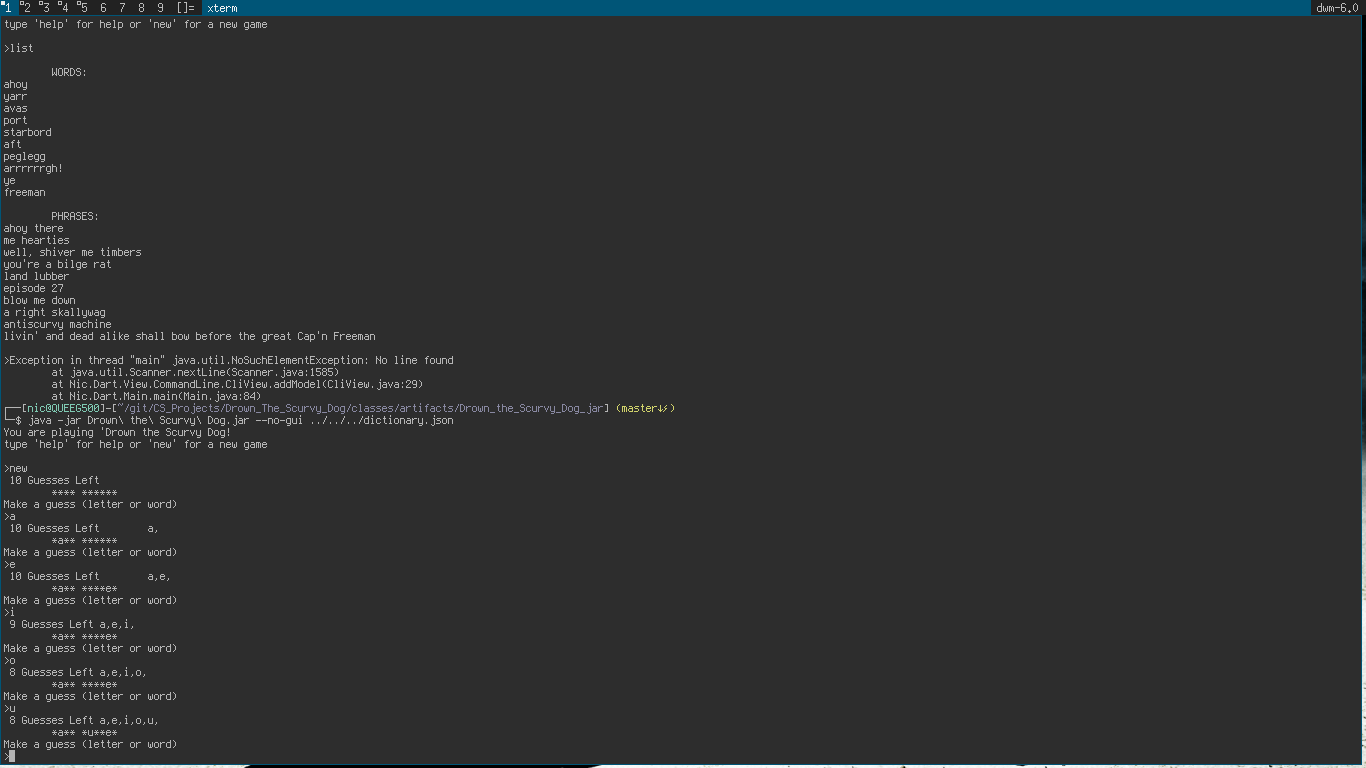
\includegraphics[scale=0.5]{./res/CliView.png}
\caption{Command Line}
\label{CliViewFinished}
\end{figure}

\begin{figure}[H]
\centering
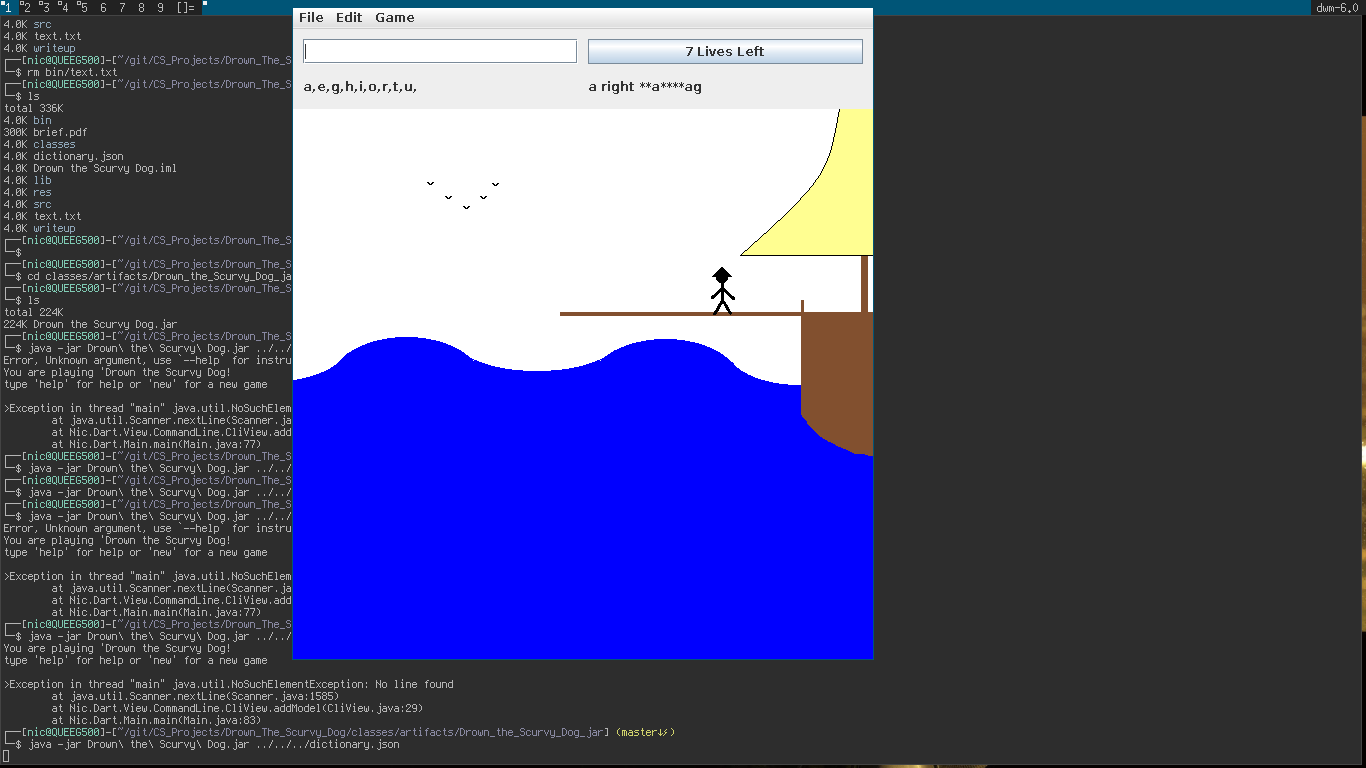
\includegraphics[scale=0.5]{./res/SwingView.png}
\caption{Swing View}
\label{SwingViewFinished}
\end{figure}

\section{Testing}

\subsection{Model Testing}

\begin{tabulary}{1\textwidth}{|L|p{10cm}|p{5cm}|p{5cm}|C|}
\hline
\textbf{ID} & \textbf{Description} & \textbf{Input} & \textbf{Expected Output} & \textbf{Pass or Fail} \\
\hline
1 & getVisible returns whole word & `a right skallywag' & `a right skallywag' & Pass \\
\hline
2 & \multirow{4}{10cm}{getHidden returns correct value with the word containing spaces, special characters and with no and some guesses made} & `arrrrrrgh!' & `**********' & Pass \\
\cline{1-1}
\cline{3-5}
3 & & `antiscurvy machine' & `********** *******' & Pass \\
\cline{1-1}
\cline{3-5}
4 & & `starbord!' with guessed charc `s' and `r' & `s**r**r**' & Pass \\
\cline{1-1}
\cline{3-5}
5 & & `livin' and dead alike shall bow before the great cap'n freeman' & guesse chars `a', `b', `c' & Pass \\
\hline
6 & guess correct and incorrect are registered correctly & `land lubber' with guessed chars `a', `b', `c' & 9 & Pass \\
\hline
7 & getLetters returns all letters guessed, correct or incorrect, excluding repeat entries & `antiscurvy machine' with guessed chars `a', `b', `c', `d' & `a,b,c,d,' & Pass \\
\hline
8 & \multirow{4}{10cm}{try char guess with upper and lower case letters and special characters} & `ahoythar' with guessed char `a' & True & Pass \\
\cline{1-1}
\cline{3-5}
9 & & `meharties' with guessed char `H' & True & Pass \\
\cline{1-1}
\cline{3-5}
10 & & `arrrrrrgh!' with guessed char `!' & True & Pass \\
\cline{1-1}
\cline{3-5}
11 & & `arrrrrrgh!' with guessed char `\%' & False & Pass \\
\hline
12 & \multirow{3}{10cm}{try word with uppercase and lowercase, with and without spaces and special chars} & `freeman' with guessed word `freeman' & True & Pass \\
\cline{1-1}
\cline{3-5}
13 & & `livin' and dead alike shall bow before the great Cap'n Freeman' with guessed word `livin' and dead alike shall bow before the great cap'n freeman' & True & Pass \\
\cline{1-1}
\cline{3-5}
14 & & `starbord' with guessed word `STARBORD' & True & Pass \\
\hline
\end{tabulary}

\begin{tabulary}{1\textwidth}{|L|p{10cm}|p{5cm}|p{5cm}|C|}
\hline
\textbf{ID} & \textbf{Description} & \textbf{Input} & \textbf{Expected Output} & \textbf{Pass or Fail} \\
\hline
15 & try word with uppercase and lowercase, with and without spaces and special chars & `antiscurvy machine' with guessed word `AnTiScUrVy MaChInE' & True & Pass \\
\hline
16 & guess with whole word completes the game & `ahoy' with guess `ahoy' & True & Pass \\
\hline
17 & guess with all letters completes the game & `ye' with guessed chars `y' and `e' & True & Pass \\
\hline
18 & guess with wrong word does not complete the game & `aft' with guessed word `asdf' & False & Pass \\
\hline
19 & guess with some letters does not complete the game & `peglegg' with guesses `p' and `e' & False & Pass \\
\hline
20 & tests if the game is considered over if 10 wrong guesses are made & `XYZ' with guessed chars `A' through `J' & True & Pass \\
\hline
21 & tests if the game is considered over if only one guessed char is made & `wheresTheRumGone?' with guessed char `p' & False & Pass \\
\hline
22 & tests if the game is considered over if a word is guessed & `isTheRumGone?' with guessed word `theRumsGoneJack!' & False & Pass \\
\hline
23 & checks fails are tallied correctly & `well blow me down!' with guessed word `blow me down!' and guessed char `p' & 2 & Pass \\
\hline



\end{tabulary}

\begin{figure}[H]
\centering
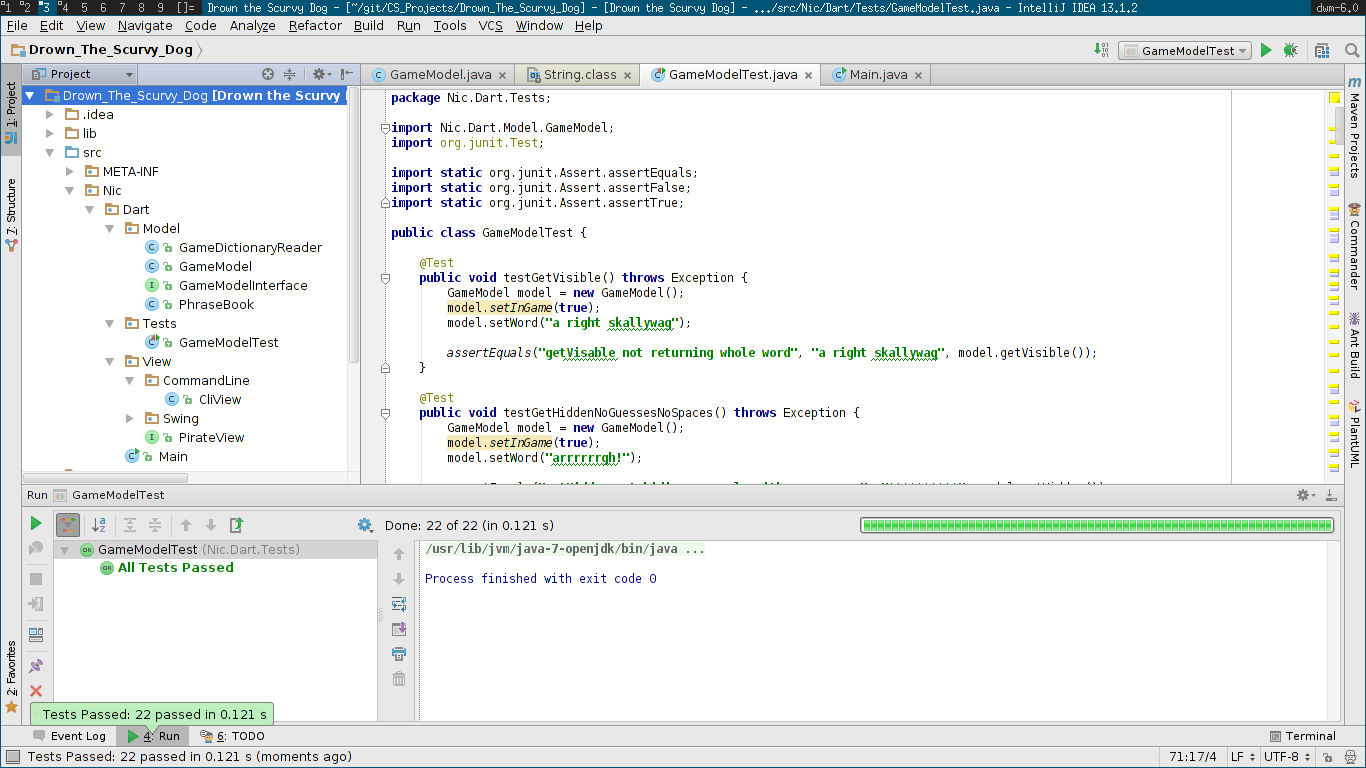
\includegraphics[scale=0.5]{./res/tests.png}
\caption{JUnit Testing Screenshot}
\label{JUnitTests}
\end{figure}

\end{landscape}

\section{Evaluation}

\subsection{Self Evaluation}

For this assignment I would give myself a mark of \textbf{71/100}, which translates to an \textbf{A grade}.

I believe this mark is an accurate representation of the amount of work I have put into the assignment. I would estimate I have spent over 40 hours in total on this project, including design, research, implementation, testing/debugging and documentation.

I feel my solution to this problem is for the most part maintainable and expendable. I would have preferred to stick more closely to the principles of MVC. 

I feel I could have improved 

\subsection{Running instructions}

For best results, run the jar:

If the dictionary is in the same directory as the jar file, then simply use
\begin{quote}
\$ java -jar DrownTheScurvyDog.jar
\end{quote}

else use:
\begin{quote}
\$ java -jar DrownTheScurvyDog.jar \textless path for dictionary.json\textgreater
\end{quote}

To run the source directly, use
\begin{quote}
\$ java -classpath bin/:lib/gson-2.2.4.jar Nic.Dart.Main
\end{quote}




\vspace{\baselineskip}

Whilst completing this assignment, I have increased my knowledge and experience in developing Java Swing applications, use and implementation of the MVC programming paradigm and the appropriate use of packages to separate out classes/files.
\section{External resources used}

\begin{enumerate}
\item Google's Gson library for parsing, reading and producing Json \url{https://code.google.com/p/google-gson/}
\item IDEA's Intellij IDEA (instead of eclipse) \url{http://www.jetbrains.com/idea/} 
\item Lecture presentations and worksheets on Blackboard
\item GenMyModel for UML/Class/Package diagrams \url{https://app.genmymodel.com/}
\end{enumerate}

\end{document}